\chapter{Results and Discussions}
%%%%%%%%%%%%%%%%%%%%%%%%%%%%%%%%%%%%%%%%%%%%%%%%%%%%%%%%%%%%
%%%%%%%%%%%%%%%%%%%%  NEW SECTION   %%%%%%%%%%%%%%%%%%%%%%%%
%%%%%%%%%%%%%%%%%%%%%%%%%%%%%%%%%%%%%%%%%%%%%%%%%%%%%%%%%%%%
\setcounter{equation}{0}
\section{Performance Evaluation}
The use case diagram, given in figure 4.1, for the proposed system is described as follows: The Different users in the system are Requestor, Donor and Administrator. Administrator maintains the information about blood availability in blood banks and, processes and validates the requests for actions raised by the Requestor; he is responsible for maintaining the database of donors and keeping the log of blood donations. Requestor is the user who raises blood requirements in the system. A Requestor can be either an individual or a blood bank. If the Requestor is a blood bank, there is no need of another registration procedure, since blood banks are already a part of the system (they are already registered users). But, if the Requestor is an individual, he/she has to go through a registration procedure, where his request is validated inorder to maintain the privacy of donors (ie, not disclosing donor details to malicious users). Requestor can search for nearby blood banks and available donors. He is also responsible for responding to donor and administrator. The third user is the Donor. He responds to the requests raised by Requestors either by accepting or rejecting them. If he accepts the request, he can contact the Requestor and the blood requirement will be satisfied and, if he rejects, that particular Donor is removed from the results and the search results will be updated.

\begin{figure}
    \centering
    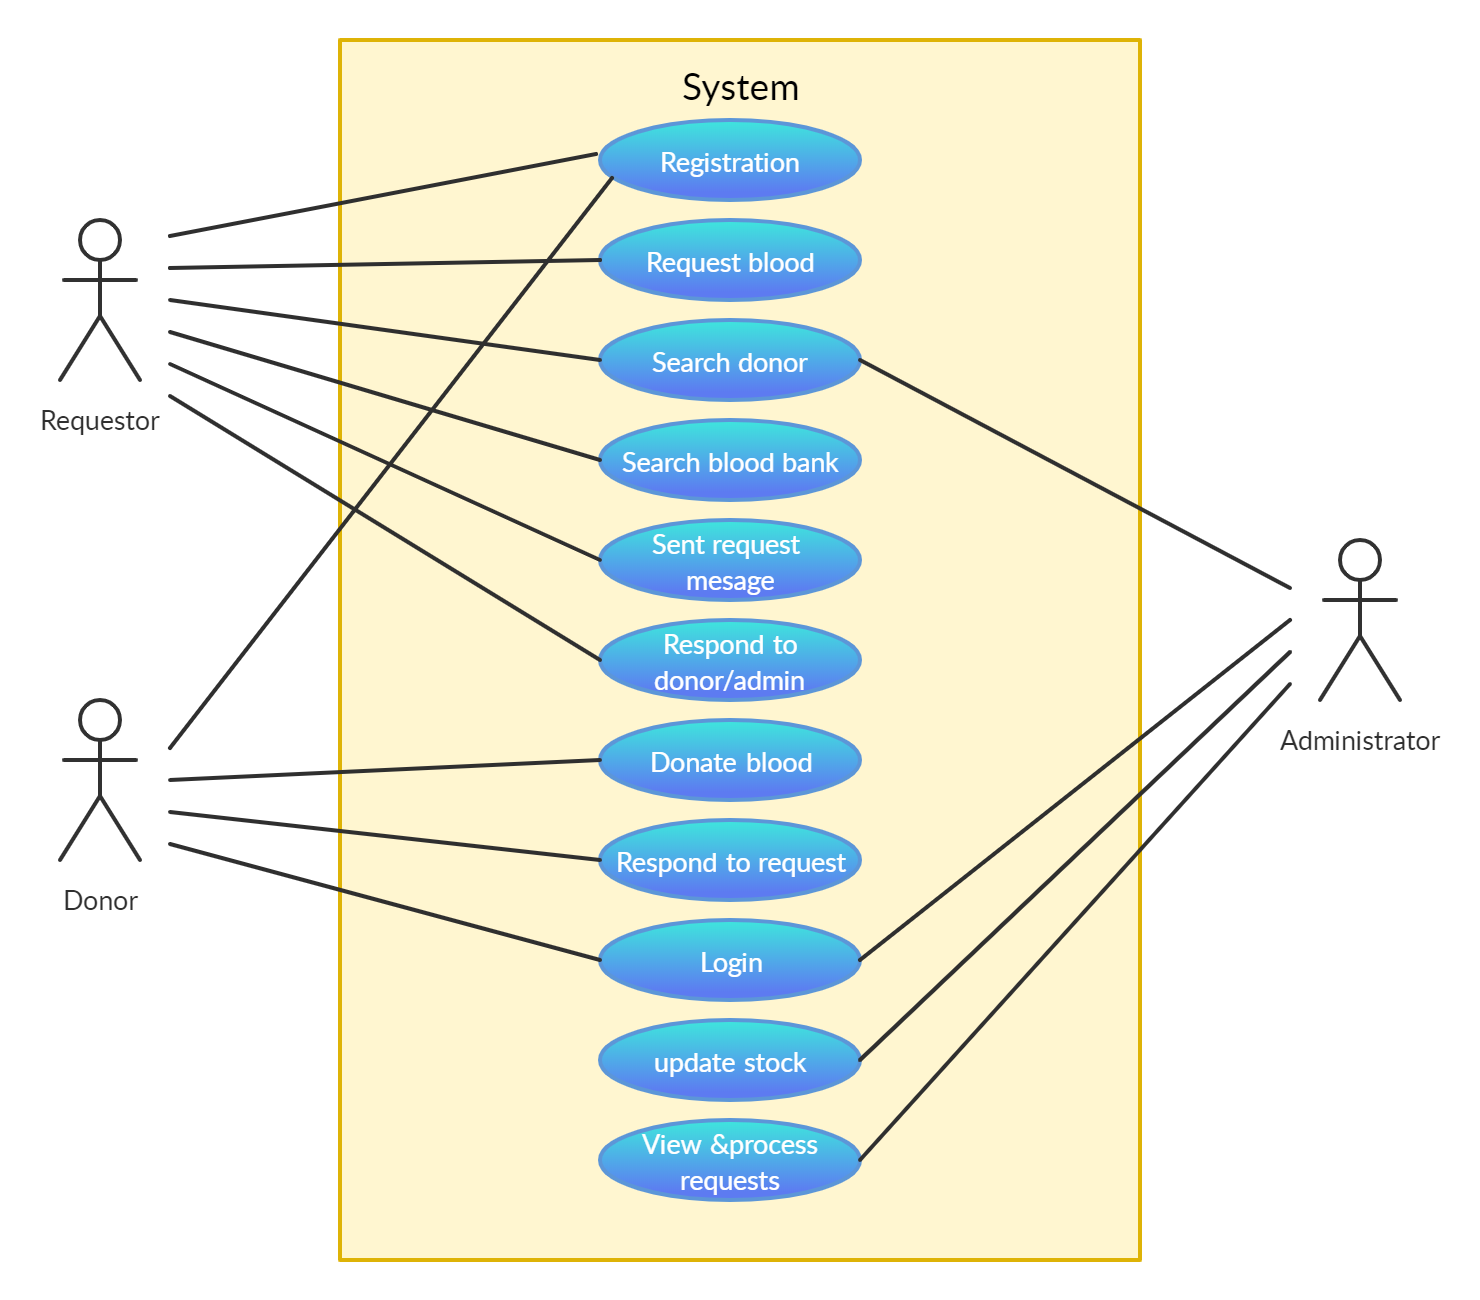
\includegraphics[width=\textwidth]{UseCase.jpg}
    \caption{Use caase diagram}

\end{figure}

\section{XXXX}
Activity diagram for processing blood requirements given in figure 4.2 is depicted  below. Requestor initiates a blood request by registering through the portal and provides the necessary information for the request. The request is validated in the server side either by the Administrator or by a 'verified' Donor. On receipt of a request, the database of available Donors and blood banks is searched and results are formulated. These results are then send back to the Requestor. Requestor selects a number of Donors and his blood request is registered on the log simultaneously. A notification is sent to those Donors selected by the Requestor. Donor recieves the request and, he can either accept or reject the request. If the Donor accepts the request, the request is verified and recorded, the Requestor will be informed that his request has been satisfied and then, donor and requestor can communicate with each other. If the Donor rejects the request, the search results gets updated by removing his name from the list. If every Donor rejects the request, the search results become empty and we have to inform the Requestor that none of the selected Donors are available so that he can select new Donors and send request to them. 
\begin{figure}
    \centering
    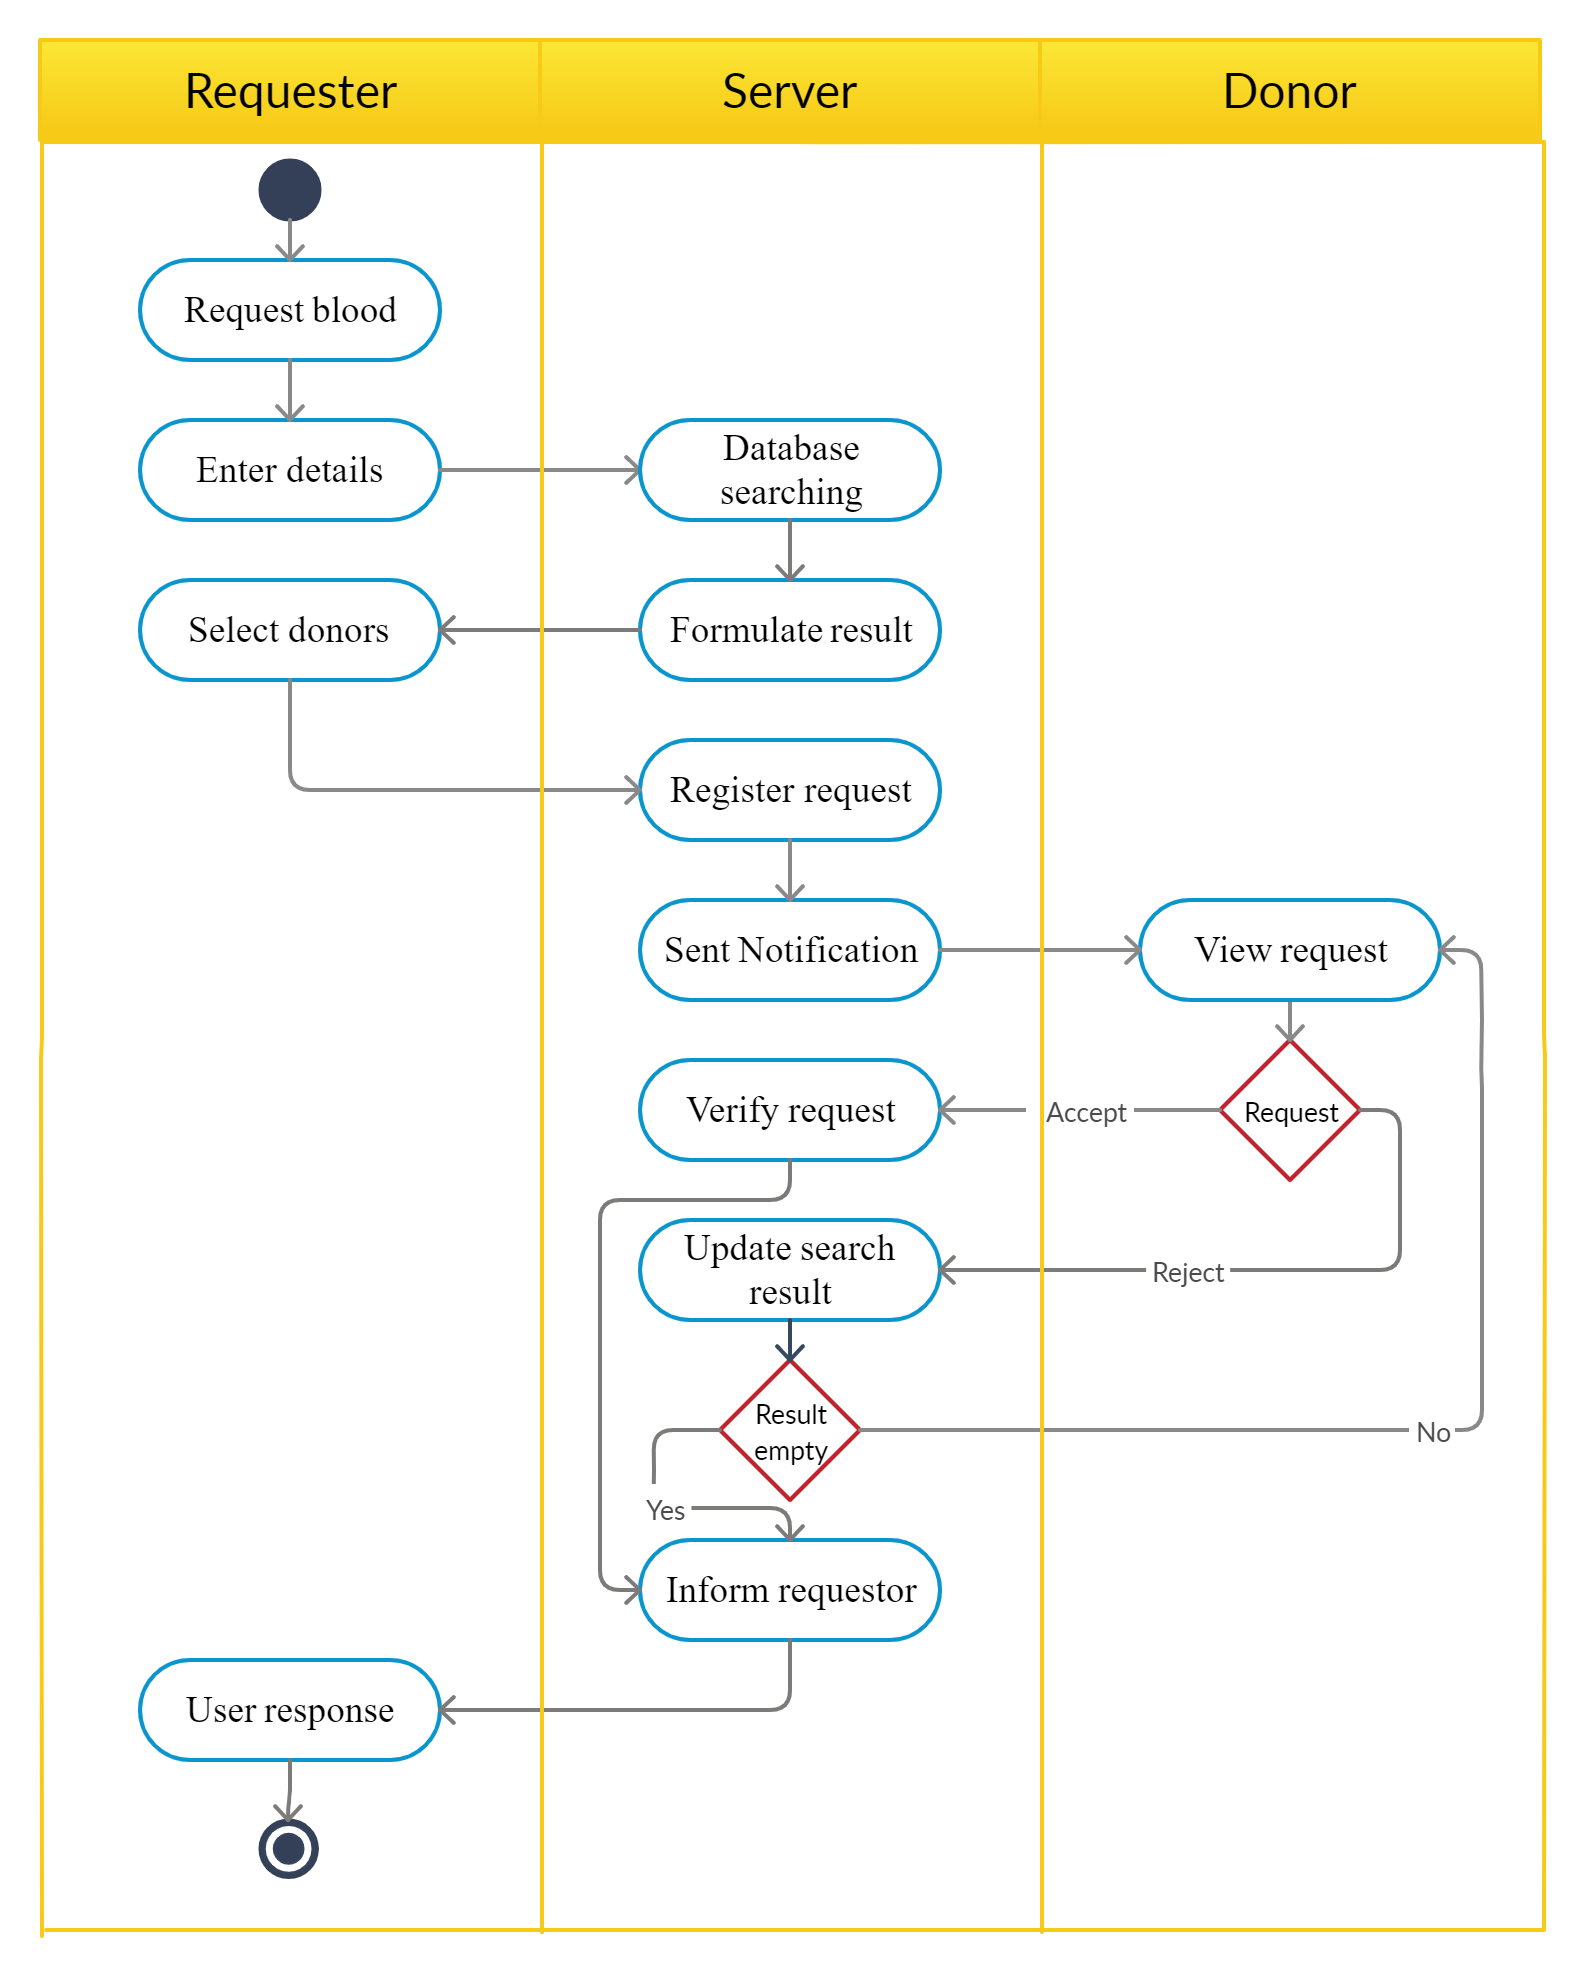
\includegraphics[width=\textwidth]{Activity.jpg}
    \caption{Activity diagram}
\end{figure}

\section{Comparison with State-of-the-Art methods}

The sequence diagram is depicted in figure 4.3. First event is the blood requirement raised by the Requestor through the web portal. On receipt of the request, we search the database for matching Donors and formulate a result. Then this result is sent to the requestor so that he can select some Donors. The system will collect the contact details of the selected donors and, notifications about the blood requirement are sent to the selected donors via emails. Based on the response of the Donor, two events are likely to happen. If the Donor accepts the request, the system will update the database with his donation status and the processed request, and the system will notify the Requestor that his blood requirement has been satisfied. Incase the Donor rejects the request system will search for other available donors and informs the Requestor about it.
 
\begin{figure}
    \centering
    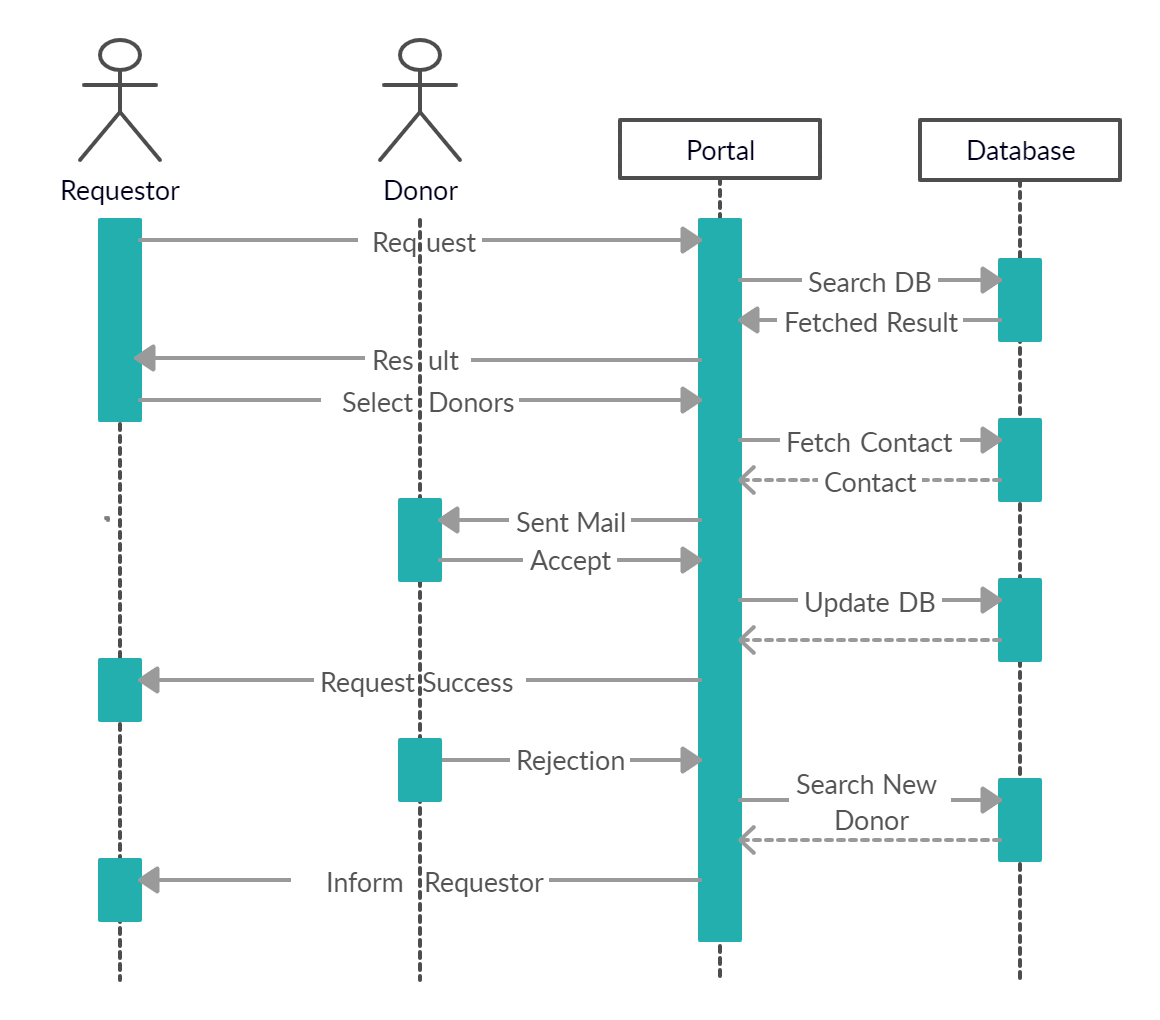
\includegraphics[width=\textwidth]{Sequence.jpg}
    \caption{Sequence diagram}
\end{figure}

\section{Discussion}


Entity relationship diagram depicts the basic structure of the database we use in our system. The ER diagram for our proposed system is given in figure 4.4 which shows the relationship between the entities of our system. We have six entities in our system which are blood banks, blood bank administrators, blood, donors, requestors and administrator. Administrator manages all the blood banks and, he is responsible for maintaining the system. He has a unique employee id. Blood bank administrators have the authority to register and verify the donors. Basic informations like age, blood group and contact details of the donor are stored in the database and every donor have a unique donor id. Blood donated by the donors are stored in the blood bank for future use. Each unit of blood has its unique unit id and expiry date for blood is also noted. Each blood banks stores a minimum amount for each blood group inorder to satisfy emergency requests. A requestor can order blood from the blood bank incase of blood requirement. Each request is stored with a request id and contact information of the requestor.

\begin{figure}[bp!]
    \centering
    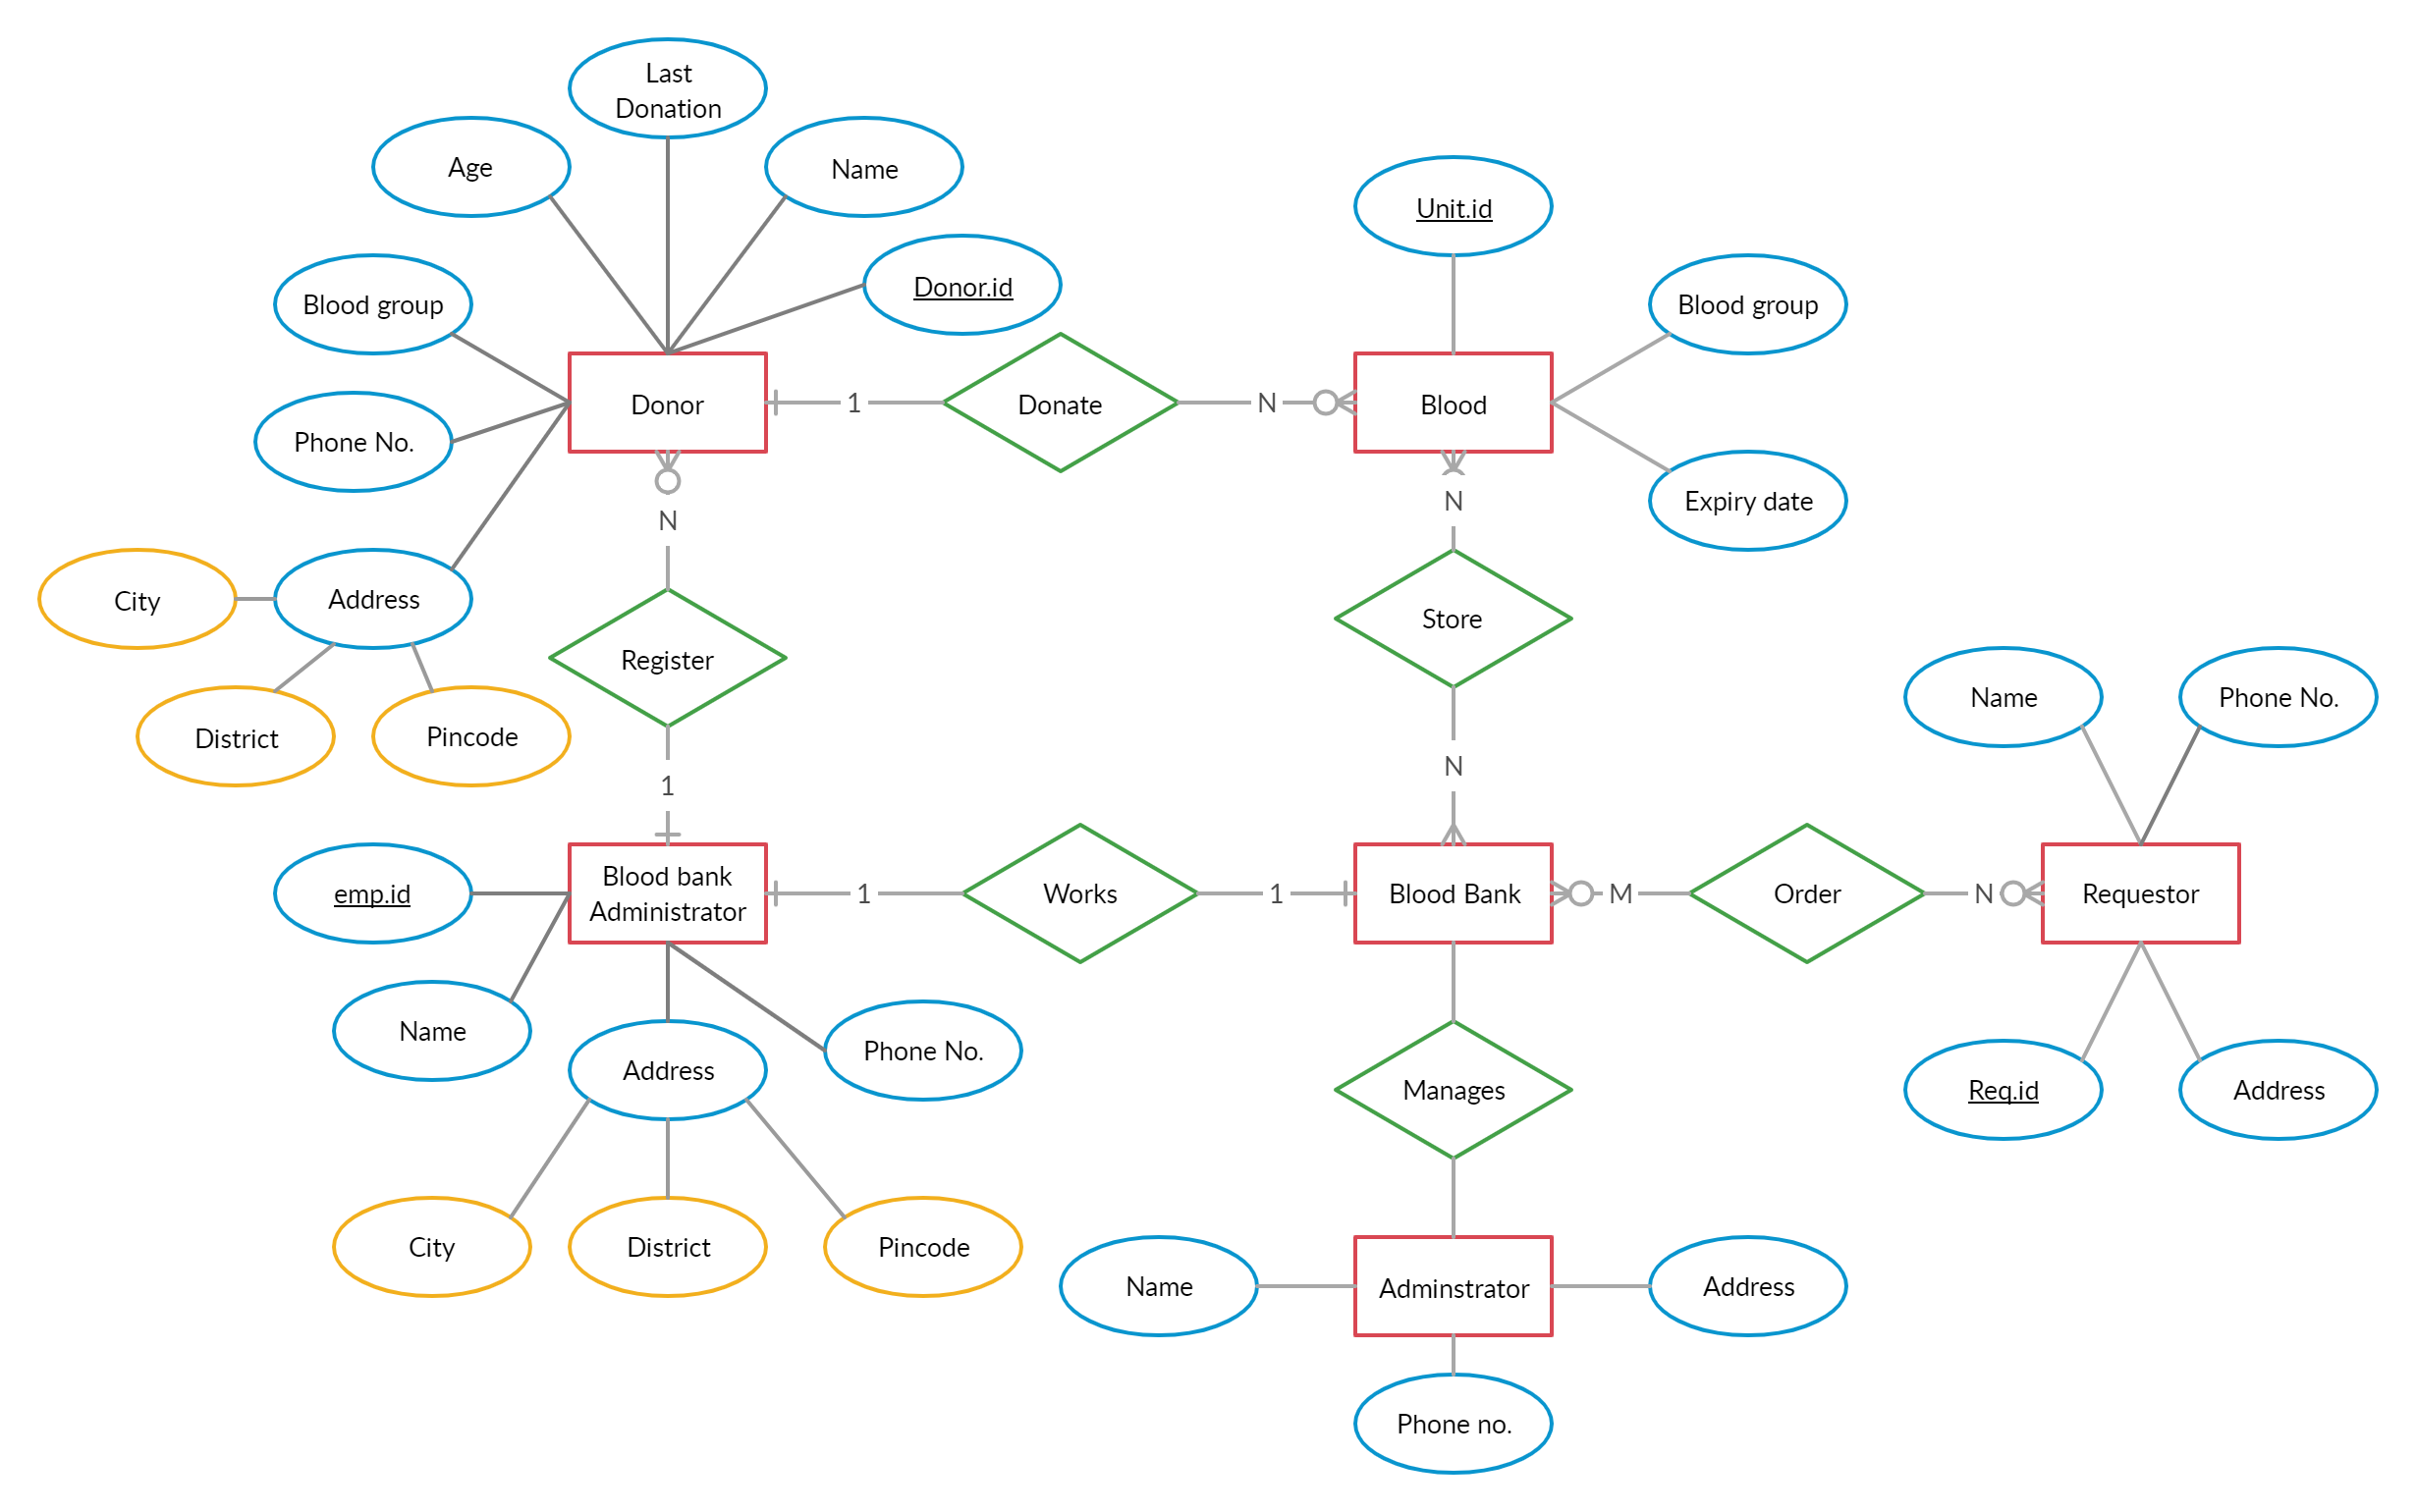
\includegraphics[width=\textwidth]{ER.jpg}
    \caption{Entity Relationship diagram}
\end{figure}

